\documentclass[conference]{IEEEtran}
\IEEEoverridecommandlockouts
\usepackage{cite}
\usepackage{amsmath,amssymb,amsfonts}
\usepackage{graphicx}
\usepackage{textcomp}
\usepackage{xcolor}
\usepackage{booktabs}
\usepackage{multirow}
\usepackage{tikz}
\usetikzlibrary{positioning,arrows.meta,shapes.geometric,fit,calc}
\usepackage{url}
\def\BibTeX{{\rm B\kern-.05em{\sc i\kern-.025em b}\kern-.08em
    T\kern-.1667em\lower.7ex\hbox{E}\kern-.125emX}}

\begin{document}

\title{Regime-Normalized Residuals and Persistence-Based Alarms for Early Wind Turbine Fault Detection on the CARE to Compare Benchmark}

% AUTHOR DETAILS ARE NOT AVAILABLE IN THE PROJECT FILES: complete before submission.
\author{\IEEEauthorblockN{Author Name(s)}
\IEEEauthorblockA{\textit{Department} \\
\textit{Institution}\\
City, Country \\
email address}
}

\maketitle

\begin{abstract}
Normal-behaviour models (NBMs) of supervisory control and data acquisition (SCADA) signals are widely used for wind turbine condition monitoring, but published evaluations rarely report how often a detector raises false alarms on healthy turbines. This paper reports a detection pipeline and digital-twin demonstrator built on Wind Farm A of the CARE to Compare benchmark, together with an evaluation of both. The pipeline fits one NBM per monitored signal, normalizes residuals with robust statistics per operating regime, accumulates evidence with exponentially weighted moving average (EWMA) and cumulative sum (CUSUM) statistics, and raises alarms through a persistence and hysteresis state machine. A diagnosis layer names the most likely component or returns an explicit unknown result. All methods were scored with the same implementation of the CARE score and with operational metrics, with alarm parameters tuned leave-one-turbine-out. The selected detector reached a CARE score of 0.637 and raised 3 false-alarm events on 10 normal datasets, against 0.576 and 14 for the residual detector of the previous project version. It detected 8 of 12 logged faults against 9 of 12, so the pre-registered target of fewer false alarms at equal recall was not met. All three gearbox failures were missed, and the component was named correctly for only 2 of 8 detections. An audit also showed that 31.3\,\% of the test rows of the earlier power forecast were present in its training data.
\end{abstract}

\begin{IEEEkeywords}
wind turbine, condition monitoring, SCADA, normal behaviour model, anomaly detection, EWMA, CUSUM, digital twin, CARE score
\end{IEEEkeywords}

\section{Introduction}
SCADA systems record 10-minute statistics of temperatures, speeds, currents and power for every utility-scale wind turbine. Because these data are already collected, residual-based monitoring of SCADA signals is an inexpensive complement to vibration-based condition monitoring \cite{tautzweinert2017review}. The usual approach trains a regression model on healthy operation, predicts each monitored signal from the operating conditions and treats persistent deviations between measurement and prediction as evidence of a developing fault \cite{schlechtingen2011comparative,chesterman2023nbm}.

The difficulty lies in the decision step. Residuals of thermal signals are autocorrelated, depend on load and ambient temperature, and contain artefacts from data errors and transient operation. A simple threshold therefore either misses slow degradations or raises many alarms on healthy turbines. Most published studies report detections on a handful of failures and seldom quantify false alarms on healthy data in a comparable way. The CARE to Compare dataset and its CARE score were introduced to address this by rewarding coverage, accuracy on normal behaviour, event-level reliability and earliness together \cite{gueck2024care}.

This work started from an existing student digital-twin project with a power forecast, a five-turbine simulation and two fault detectors evaluated on Wind Farm A. Its supervised random-forest classifier detected 8 of 12 logged faults but flagged 6 of 10 healthy datasets and named the correct fault class only once. With at most six recorded events per fault class, a more complex supervised classifier was unlikely to generalize. The work reported here therefore treats detection and diagnosis as separate problems and makes the alarm decision the main object of study. Its contributions are:
\begin{enumerate}
\item a detection pipeline combining leakage-controlled NBMs, regime-aware robust residual normalization, EWMA and CUSUM statistics and a persistence and hysteresis state machine, with a diagnosis step that may return an unknown result;
\item an evaluation of this pipeline and six other detectors on CARE to Compare Wind Farm A (version 6) under one protocol and one scorer, reporting CARE sub-scores, false-alarm events, detection delays and diagnosis accuracy with counts;
\item an audit of the earlier power forecast showing train and test leakage, and a corrected forecast with split-conformal prediction intervals;
\item a web-based digital twin that replays the real SCADA data through the same streaming monitor, keeps synthetic simulation separate from real-data evidence and shows the evaluation results in the user interface.
\end{enumerate}

\section{Related Work}
\subsection{Normal-Behaviour Modelling}
Schlechtingen and Santos compared regression-based and neural-network NBMs of SCADA temperatures for wind turbine fault detection \cite{schlechtingen2011comparative}. Bangalore and Tjernberg used neural-network NBMs of gearbox bearing temperatures and the Mahalanobis distance of the residuals to raise early warnings \cite{bangalore2015ann}. A later comparison on operational wind farms found that elastic-net regression performed about as well as LightGBM and multilayer perceptrons overall. The same study found that tree models degraded during long cool-down periods and that a robust median absolute deviation (MAD) scheme detected more failures than CUSUM, at the cost of more unexplained alarms \cite{chesterman2023nbm}. Letzgus showed that change points in about one third of SCADA signals corrupt NBM training data unless they are detected and removed \cite{letzgus2020change}. Lichtenstein \emph{et al.} modelled drivetrain temperatures with empirical physics-based NBMs on high-resolution data \cite{lichtenstein2025physics}. These studies agree that NBMs can expose degradation, but they evaluate on turbine-specific failure sets with different scoring rules, so the false-alarm cost of each design is hard to compare.

\subsection{Alarm Logic and Diagnosis}
EWMA \cite{roberts1959ewma,lucas1990ewma} and CUSUM \cite{page1954cusum} charts are standard tools for detecting persistent small shifts, and both have been applied to NBM residuals \cite{chesterman2023nbm}. Wind-specific guidance on their parameters is scarce. The CARE benchmark uses a criticality counter that requires about 12 hours of net anomalous behaviour before an event counts as detected \cite{gueck2024care}. For diagnosis, Roelofs \emph{et al.} proposed ARCANA, which attributes autoencoder anomalies to individual features \cite{roelofs2021arcana}. Few studies report diagnosis accuracy separately from detection, or allow a monitor to decline a diagnosis.

\subsection{Benchmark and Research Gap}
CARE to Compare contains 95 datasets from 36 turbines in three farms, with 44 labelled anomaly events in the published paper \cite{gueck2024care}. Version 6 of the data contains 45 anomaly and 50 normal datasets \cite{gueck2025zenodo}. The reference autoencoder scored 0.66 over all datasets, a random strategy 0.5, and an isolation forest below 0.5 \cite{gueck2024care}. We did not find a peer-reviewed per-farm CARE result for Wind Farm A under the official protocol. The gap addressed here is therefore not a new detector family but an evaluation of an established, interpretable residual pipeline in which alarm persistence, false-alarm counts and diagnosis are reported next to the CARE score and compared with the earlier detectors of this project on identical data.

\section{Data and Evaluation Protocol}
\subsection{Dataset}
Wind Farm A comprises five onshore turbines in Portugal with 86 features at 10-minute resolution, from the EDP open-data platform \cite{gueck2024care}. Its 22 datasets each contain a training period and a prediction period; 12 prediction periods contain a logged fault (gearbox 3, generator bearing 2, hydraulic group 6, transformer 1) and 10 are normal. We used version 6 of the data (DOI 10.5281/zenodo.15846963) \cite{gueck2025zenodo}. Following the dataset documentation, only per-timestamp average signals were used, because the minimum, maximum and standard-deviation channels contain implausible values. Pitch angles were unwrapped from the 0 to 360\,\textdegree{} range. Status labels were used only to select healthy training rows (status 0 or 2) and never as model inputs.

\subsection{Splits and Parameter Selection}
For each dataset, NBMs were fitted on the first 80\,\% of its healthy training rows. The last 20\,\% served as a chronological validation split for residual statistics and statistic scales. Prediction rows were never used for fitting. Monitoring ran causally from two days before the prediction window. Alarm parameters, and the score thresholds of the isolation forest and autoencoder baselines, were chosen leave-one-turbine-out: settings were selected by maximizing CARE on the datasets of four turbines and applied to the fifth, and the five held-out folds were pooled.

\subsection{Metrics}
The CARE score was computed as in the reference implementation \cite{efd2026}. Let $p_t\in\{0,1\}$ be the point prediction. The criticality counter is
\begin{equation}
c_t=\begin{cases}\min(c_{t-1}+1,\,1000), & p_t=1\\ \max(c_{t-1}-1,\,0), & p_t=0\end{cases}\label{eq:crit}
\end{equation}
and an event is detected when $\max_t c_t\geq 72$ in (\ref{eq:crit}). Coverage is the mean pointwise $F_{0.5}$ score over anomaly events, accuracy the mean true-negative rate over normal events, reliability the event-level $F_{0.5}$ score and earliness a weighted score over the event window. With these sub-scores,
\begin{equation}
\mathrm{CARE}=\begin{cases}\bar{A}, & \bar{A}\leq 0.5\\ \dfrac{C+E+R+2\bar{A}}{5}, & \text{otherwise}\end{cases}\label{eq:care}
\end{equation}
where $C$, $E$, $R$ and $\bar{A}$ denote coverage, earliness, reliability and mean accuracy; the score in (\ref{eq:care}) is set to 0 if no event is detected \cite{gueck2024care}. The reference code starts the decay of the earliness weights at one quarter of the event window, whereas the paper text describes one half; we followed the code. Because CARE scores point predictions, we also report operational metrics: an event counts as detected when an alarm is active inside its logged window, false-alarm events are alarm episodes in the prediction windows of normal datasets, and delays are measured from the logged event start. Normal prediction data total 5.95 turbine-months. The Farm A event starts are derived from a fault logbook, so delays are approximate.

\section{Detection Pipeline}
Fig.~\ref{fig:arch} shows the processing chain. The same code runs in batch mode for the benchmark and in streaming mode for replay and simulation; a unit test checks that both modes give identical states.

\begin{figure*}[t]
\centering
\resizebox{\textwidth}{!}{%
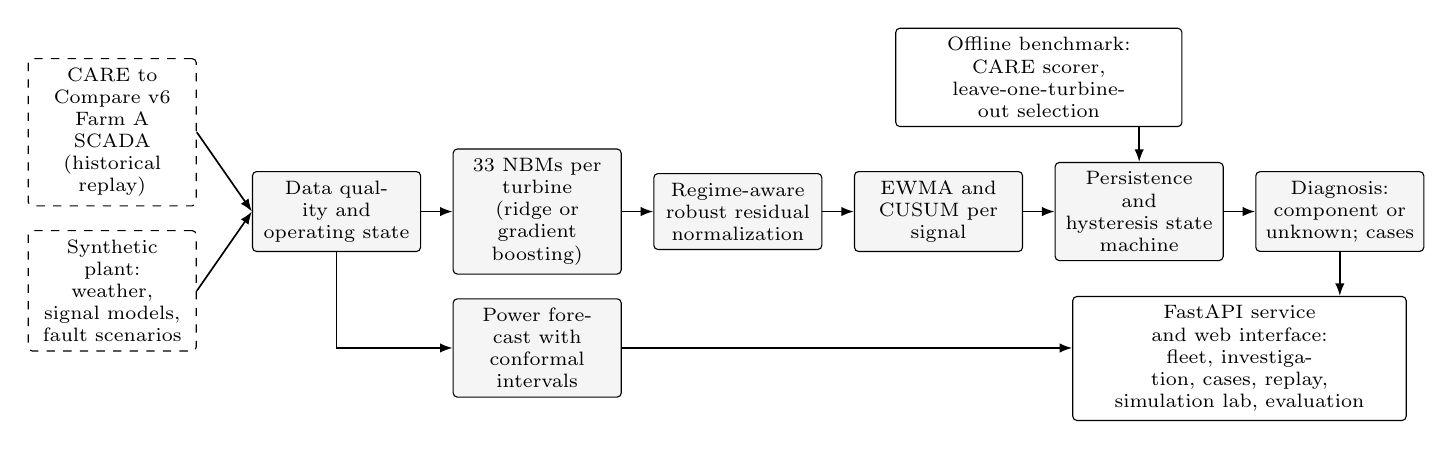
\begin{tikzpicture}[
  font=\scriptsize, node distance=3mm and 4mm,
  blk/.style={draw, rounded corners=1.5pt, align=center, minimum height=8.5mm, text width=19mm, fill=gray!8},
  src/.style={blk, fill=white, dashed},
  app/.style={blk, fill=white},
  arr/.style={-{Latex[length=1.6mm]}, semithick}]
\node[src] (care) {CARE to Compare v6\\Farm A SCADA\\(historical replay)};
\node[src, below=of care] (sim) {Synthetic plant:\\weather, signal models,\\fault scenarios};
\coordinate (srcmid) at ($(care.east)!0.5!(sim.east)$);
\node[blk, right=7mm of srcmid] (dq) {Data quality and\\operating state};
\node[blk, right=of dq] (nbm) {33 NBMs per\\turbine (ridge or\\gradient boosting)};
\node[blk, right=of nbm] (norm) {Regime-aware\\robust residual\\normalization};
\node[blk, right=of norm] (stat) {EWMA and\\CUSUM per\\signal};
\node[blk, right=of stat] (sm) {Persistence and\\hysteresis state\\machine};
\node[blk, right=of sm] (dx) {Diagnosis:\\component or\\unknown; cases};
\node[blk, below=of nbm] (fc) {Power forecast with\\conformal intervals};
\coordinate (topmid) at ($(stat.north)!0.5!(sm.north)$);
\coordinate (botmid) at ($(sm.south)!0.5!(dx.south)$);
\node[app, above=5mm of topmid, text width=34mm] (bench) {Offline benchmark: CARE scorer,\\leave-one-turbine-out selection};
\node[app, below=5mm of botmid, text width=40mm] (ui) {FastAPI service and web interface:\\fleet, investigation, cases, replay,\\simulation lab, evaluation};
\draw[arr] (care.east) -- (dq.west);
\draw[arr] (sim.east) -- (dq.west);
\draw[arr] (dq) -- (nbm);
\draw[arr] (nbm) -- (norm);
\draw[arr] (norm) -- (stat);
\draw[arr] (stat) -- (sm);
\draw[arr] (sm) -- (dx);
\draw[arr] (dq.south) |- (fc.west);
\draw[arr] (bench.south -| sm.north) -- (sm.north);
\draw[arr] (dx.south) -- (dx.south |- ui.north);
\draw[arr] (fc.east) -- (fc.east -| ui.west);
\end{tikzpicture}}
\caption{Architecture of the implemented system. Real-data replay and the synthetic plant enter the same monitoring chain; the offline benchmark selects the alarm parameters used by the state machine.}
\label{fig:arch}
\end{figure*}

\subsection{Data Quality and Operating State}
Each raw signal is checked for missing values, physically implausible ranges, implausible jumps between consecutive samples and flatlines (for example, a temperature unchanged for 48 hours). A row is rated bad when a core signal (wind speed, power or ambient temperature) fails or when at least 30\,\% of the signals fail; bad rows produce the state \emph{unknown} rather than an alarm. The operating state (production, curtailed, idle or stopped) is inferred from power, wind speed, pitch and a binned power curve. Idle and stopped rows are not judged.

\subsection{Normal-Behaviour Models}
One model is fitted for each of 33 targets grouped into ten components: gearbox, generator bearings, generator windings, transformer, hydraulic group, hub and pitch, converter, nacelle cabinets, electrical balance and power performance. Targets include raw temperatures and physically motivated derived signals, such as the drive-end minus non-drive-end generator bearing temperature, gearbox bearing minus oil temperature, phase spreads and hydraulic oil minus nacelle temperature. Inputs describe operating conditions only: wind speed, power and its 1 to 12 hour rolling means for thermal inertia, ambient and nacelle temperature, rotor and generator speed, and time of day. A target never receives its own sensors, sibling sensors of the same component or inputs from its correlation group, and any remaining input with absolute correlation above 0.98 to the target is dropped. Each target is fitted with ridge regression and with histogram-based gradient boosting \cite{friedman2001gbm}; after one round of trimming residuals beyond four robust standard deviations, gradient boosting is kept only if it lowers the validation residual spread by more than 10\,\%. It was retained for 627 of 726 target models.

\subsection{Regime-Aware Residual Normalization}
For target $j$ with measurement $y_{t,j}$ and prediction $\hat{y}_{t,j}$, the residual is $r_{t,j}=y_{t,j}-\hat{y}_{t,j}$. Operating regimes $b$ are formed from five power bins and ambient-temperature terciles. On the validation split, the median $m_{b,j}$ and the robust scale $\sigma_{b,j}=1.4826\,\mathrm{MAD}$ \cite{rousseeuw1993mad} are estimated per regime and shrunk toward the global values with weight $w=n/(n+100)$ for a bin with $n$ rows. A physical floor (for example 0.5\,K for temperatures) prevents overconfident scales. The standardized residual is
\begin{equation}
z_{t,j}=d_j\,\frac{r_{t,j}-m_{b(t),j}}{\sigma_{b(t),j}},\label{eq:z}
\end{equation}
clipped to $\pm 8$, where $d_j=1$ for temperatures (hotter is worse), $d_j=-1$ for power (lower is worse) and two-sided targets such as pitch keep their sign.

\subsection{Temporal Statistics and Alarm State Machine}
Each target is tracked by an EWMA and a one-sided CUSUM \cite{roberts1959ewma,page1954cusum}:
\begin{align}
e_{t,j}&=\lambda z_{t,j}+(1-\lambda)\,e_{t-1,j},\label{eq:ewma}\\
S_{t,j}&=\max\!\left(0,\;S_{t-1,j}+z_{t,j}-k\right).\label{eq:cusum}
\end{align}
Because temperature residuals are strongly autocorrelated, the usual independent-sample control limits do not apply. Both statistics are therefore divided by their 99.5th percentile on the validation split; the EWMA scale is floored at the independent-sample value $2.576\sqrt{\lambda/(2-\lambda)}$ \cite{lucas1990ewma}, and the CUSUM is bounded at $1.5h$ so that it recovers after a deviation ends. Statistics freeze on rows that are not judged. A component's statistic is the maximum over its targets, and the turbine statistics $\bar{E}_t$ and $\bar{S}_t$ are the maxima over components.

Fig.~\ref{fig:flow} shows the state machine. A step is a hit when $\bar{E}_t>L$ or $\bar{S}_t>h$. Thirty-six consecutive hits (6\,h) raise a warning and open a case; 144 consecutive hits with both statistics above their limits escalate it to a fault. A case closes only after both statistics have stayed below half of their limits for 144 steps (24\,h). The selected parameters were $\lambda=0.1$, $L=2$, $k=1$ and $h=3$, chosen identically in four of the five folds; the fold holding out turbine 10 chose $\lambda=0.02$ and $L=3$.

\begin{figure}[t]
\centering
\resizebox{\columnwidth}{!}{%
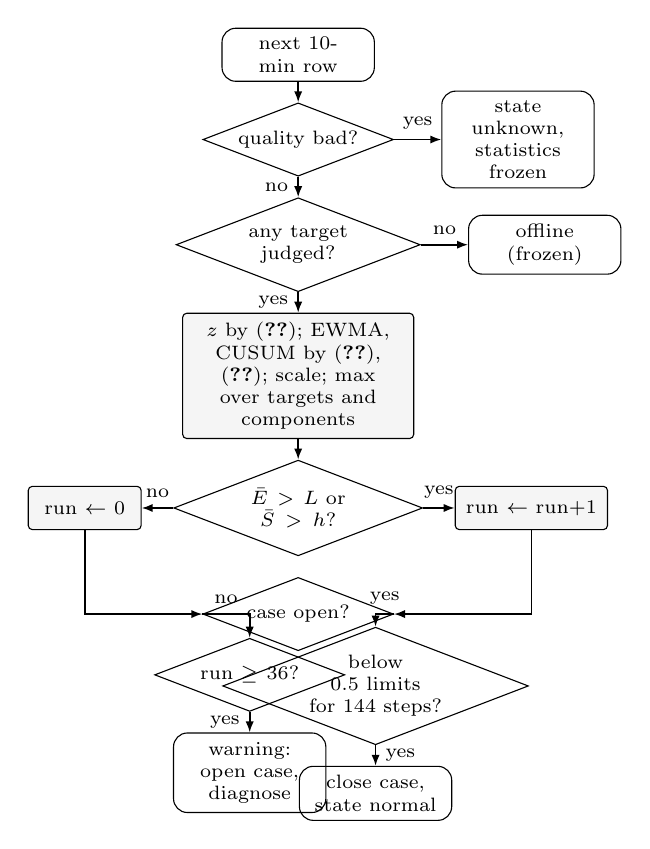
\begin{tikzpicture}[
  font=\scriptsize, node distance=2.6mm,
  proc/.style={draw, rounded corners=1.5pt, align=center, text width=27mm, minimum height=5.5mm, fill=gray!8},
  dec/.style={draw, diamond, aspect=2.6, align=center, inner sep=0.6pt, text width=17mm},
  term/.style={draw, rounded corners=5pt, align=center, text width=17mm, minimum height=5mm},
  arr/.style={-{Latex[length=1.4mm]}, semithick}]
\node[term] (in) {next 10-min row};
\node[dec, below=of in] (q) {quality bad?};
\node[term, right=6mm of q] (unk) {state unknown,\\statistics frozen};
\node[dec, below=of q] (j) {any target\\judged?};
\node[term, right=6mm of j] (off) {offline\\(frozen)};
\node[proc, below=of j] (z) {$z$ by (\ref{eq:z}); EWMA, CUSUM by (\ref{eq:ewma}), (\ref{eq:cusum}); scale; max over targets and components};
\node[dec, below=of z] (hit) {$\bar{E}>L$ or\\$\bar{S}>h$?};
\node[proc, right=4mm of hit, text width=17mm] (run) {run $\leftarrow$ run$+1$};
\node[proc, left=4mm of hit, text width=12mm] (rst) {run $\leftarrow 0$};
\node[dec, below=of hit] (lv) {case open?};
\node[dec, below left=3mm and -6mm of lv] (p) {run $\geq 36$?};
\node[term, below=of p] (w) {warning: open case, diagnose};
\node[dec, below right=3mm and -6mm of lv] (cl) {below $0.5$ limits\\for 144 steps?};
\node[term, below=of cl] (c) {close case,\\state normal};
\draw[arr] (in) -- (q);
\draw[arr] (q) -- node[above]{yes} (unk);
\draw[arr] (q) -- node[left]{no} (j);
\draw[arr] (j) -- node[above]{no} (off);
\draw[arr] (j) -- node[left]{yes} (z);
\draw[arr] (z) -- (hit);
\draw[arr] (hit) -- node[above]{yes} (run);
\draw[arr] (hit) -- node[above]{no} (rst);
\draw[arr] (run.south) |- (lv.east);
\draw[arr] (rst.south) |- (lv.west);
\draw[arr] (lv) -| node[above, pos=0.25]{no} (p);
\draw[arr] (lv) -| node[above, pos=0.25]{yes} (cl);
\draw[arr] (p) -- node[left]{yes} (w);
\draw[arr] (cl) -- node[right]{yes} (c);
\end{tikzpicture}}
\caption{Per-step alarm logic. Without an open case, a hit or a statistic above 70\,\% of its limit that has not persisted gives the state watch. With an open case, 144 consecutive hits with both statistics above their limits escalate the warning to a fault. The loop repeats for every row.}
\label{fig:flow}
\end{figure}

\subsection{Diagnosis}
When a case opens, the component evidence over the deviation window (at least 6\,h, at most 3 days) is ranked. The diagnosis is \emph{unknown} when the evidence is weak, when the runner-up component is within 25\,\% of the leader, when several unrelated components deviate together, or when more than 30\,\% of the window has bad data quality. Each case lists the supporting signals with observed value, expected value, standardized residual and contribution. No confidence value is reported, because 12 events are too few to calibrate one.

\subsection{Power Forecast and Prediction Intervals}
The expected power is predicted with gradient boosting from wind speed and its powers, the density-corrected wind speed (air density from ambient temperature at standard pressure), the 1-hour standard deviation and change of wind speed, wind direction and time of day, and compared with a binned physics power curve. Prediction intervals are split-conformal \cite{lei2018conformal}: the empirical quantile of absolute calibration residuals is computed separately for four wind-speed regimes at nominal levels of 80\,\% and 95\,\%.

\section{Digital-Twin Implementation}
An industrial digital twin is usually defined by a continuous, bidirectional link between a virtual model and its physical asset \cite{tao2019dt}. The system described here has no connection to an operating turbine; it is a monitoring demonstrator that replays recorded data and simulates synthetic turbines. The pipeline is a Python package served by a FastAPI application, with a browser interface that requires no build step. The interface has views for the fleet (including a three-dimensional farm model), turbine investigation (observed and expected signals with bands, EWMA and CUSUM traces, state timeline and evidence), case management with analyst feedback, historical replay, a simulation laboratory and model evaluation.

The replay mode streams the real prediction windows of all 22 datasets through the monitor and marks the logged event window and the first alarm. The simulation mode generates synthetic SCADA rows for five turbines from per-signal regression models trained on each real turbine's healthy training data, with first-order autoregressive noise and correlated phase noise. A library of 17 seeded scenarios (nine component faults, three performance faults and five sensor faults) modifies these rows with configurable severity, ramp and duration. Because the synthetic signals are generated one by one, their cross-correlations differ from the real turbines. At each reset the twin is therefore commissioned on six simulated healthy days: signal offsets are removed, simulated power follows the twin's own power model, and the residual normalization is re-estimated on synthetic data. This commissioning affects only the simulation. Ground truth of injected scenarios is shown only in a separate test-oracle view, and simulation results are not used as evidence of real-data accuracy.

\section{Results}
\subsection{Detection on Real Data}
Table~\ref{tab:bench} compares all methods on the 22 held-out prediction windows. The legacy random forest was re-run with leave-one-group-out cross-validation; the legacy residual detector was scored from its saved outputs, and its settings had been chosen on the same 22 datasets.

\begin{table*}[t]
\caption{Held-out results on CARE to Compare Wind Farm A (version 6): 12 anomaly and 10 normal prediction windows}
\label{tab:bench}
\centering
\footnotesize
\setlength{\tabcolsep}{4.2pt}
\resizebox{\textwidth}{!}{%
\begin{tabular}{@{}llcccccccccc@{}}
\toprule
Method & Type & CARE & Cov. & Acc. & Rel. & Earl. & Detected & FA events & FA per & Normal sets & Delay med./p90 \\
 & & & & & & & (of 12) & (normal) & turb.-month & flagged & (h) \\
\midrule
Random forest classifier (legacy) & baseline & 0.614 & 0.340 & 0.935 & 0.673 & 0.187 & 8 & 27 & 4.54 & 5/10 & 20.6 / 82.5 \\
Residual detector (legacy) & baseline & 0.576 & 0.256 & 0.951 & 0.625 & 0.097 & 9 & 14 & 2.35 & 7/10 & 94.2 / 241.6 \\
Isolation forest \cite{liu2008iforest} & baseline & 0.520 & 0.295 & 0.911 & 0.357 & 0.127 & 2 & 2 & 0.34 & 2/10 & 163.8 / 290.5 \\
MLP autoencoder & baseline & 0.644 & 0.414 & 0.925 & 0.781 & 0.174 & 5 & 0 & 0.00 & 0/10 & 28.2 / 90.5 \\
NBM + threshold & variant & 0.584 & 0.448 & 0.859 & 0.568 & 0.185 & 12 & 1018 & 171.2 & 10/10 & 2.1 / 8.0 \\
NBM + EWMA & variant & 0.549 & 0.493 & 0.754 & 0.486 & 0.257 & 12 & 280 & 47.09 & 10/10 & 7.8 / 76.4 \\
NBM + CUSUM & variant & 0.588 & 0.309 & 0.923 & 0.577 & 0.205 & 7 & 14 & 2.35 & 6/10 & 102.0 / 275.2 \\
NBM + EWMA + CUSUM, persistence tuned & variant & 0.582 & 0.349 & 0.823 & 0.667 & 0.249 & 7 & 5 & 0.84 & 4/10 & 104.2 / 218.7 \\
NBM + EWMA + CUSUM, fixed persistence & selected & 0.637 & 0.380 & 0.896 & 0.750 & 0.261 & 8 & 3 & 0.51 & 3/10 & 106.0 / 302.2 \\
\bottomrule
\end{tabular}}
\end{table*}

The selected detector reduced false-alarm events from 14 to 3 (79\,\%) relative to the legacy residual detector and raised its CARE score from 0.576 to 0.637, but it detected 8 rather than 9 events. The target fixed before the experiments (at least 25\,\% fewer false-alarm events at no lower event recall) was therefore not met. One event corresponds to about 8 percentage points of recall, so differences of one event are within the uncertainty of this benchmark. The autoencoder baseline reached the highest CARE score (0.644) without false alarms, but detected only 5 events and cannot name a component.

Fig.~\ref{fig:tradeoff} shows the trade-off between detections and false alarms. A threshold on the standardized residual alone, or EWMA alone, detected every event but produced 1018 and 280 alarm episodes on normal data, which would be unusable in operation. Their CARE scores (0.584 and 0.549) remain moderate because CARE scores point predictions and does not count repeated alarms. Persistence and hysteresis removed most of this chatter. Letting the leave-one-turbine-out search also choose persistence and cooldown (432 settings) produced unstable fold choices and a worse held-out result than fixing them at 6\,h and 24\,h.

\begin{figure}[t]
\centering
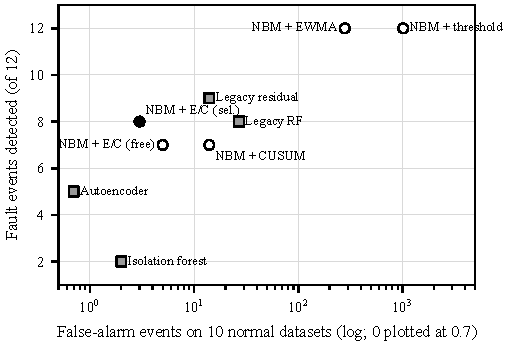
\includegraphics[width=\columnwidth]{figures/tradeoff.pdf}
\caption{Detected fault events versus false-alarm events on normal datasets (held-out). Squares: baselines; circles: NBM variants; filled circle: selected detector. E/C denotes EWMA and CUSUM.}
\label{fig:tradeoff}
\end{figure}

The missed events were all three gearbox failures (datasets 10, 51 and 72) and one hydraulic event (dataset 26). No gearbox temperature residual left its validation range within these windows. On dataset 10 an alarm opened and cleared before the logged window and was counted as a pre-event alarm. The three false alarms occurred on normal datasets 17 (a sustained hydraulic-oil residual), 24 (generator bearings) and 38 (converter). Every configuration sensitive enough to detect eight or more faults also alarmed on dataset 17, which may contain an unlogged deviation but is counted as a false alarm. Delays were long (median 106\,h after the logged event start), because several detections occurred late in the 7 to 14 day windows.

Fig.~\ref{fig:replay} shows a detected hydraulic event (dataset 22) replayed through the streaming monitor. The hydraulic oil temperature, relative to the nacelle temperature, rose above its expected value about two hours before the logged start. The CUSUM crossed its limit on the evening of the first day, and the case opened after 6\,h of persistence, 12.8\,h after the logged start, with the hydraulic group as the leading component (42\,\% of the evidence, against 24\,\% for the gearbox).

\begin{figure}[t]
\centering
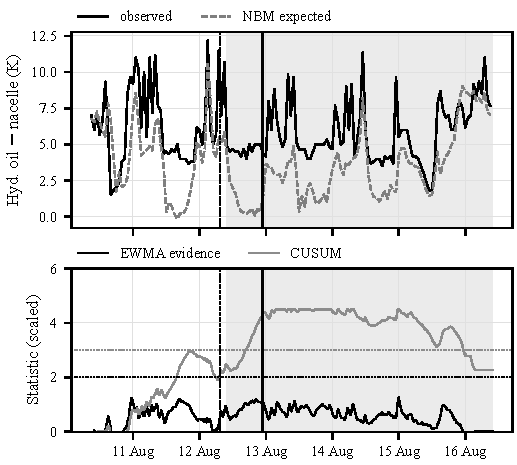
\includegraphics[width=\columnwidth]{figures/replay22.pdf}
\caption{Replay of dataset 22 (hydraulic group). Top: hourly mean of hydraulic oil minus nacelle temperature and NBM expectation. Bottom: scaled EWMA evidence and CUSUM of the hydraulic group with limits (dotted). Shaded: logged event window; dashed line: deviation start; solid line: alarm.}
\label{fig:replay}
\end{figure}

\subsection{Diagnosis}
Of the 8 detected events, the component was correct twice (generator bearings in dataset 0, hydraulic group in dataset 22), unknown once (dataset 45) and wrong five times. Hydraulic events often appeared first in nacelle-cabinet, converter or generator-bearing residuals. Component recall over all logged events was 1 of 2 for generator bearings, 1 of 6 for the hydraulic group and 0 for the gearbox and transformer classes. These figures do not support claims of reliable component diagnosis.

\subsection{Power Forecast}
The audit of the earlier forecast found that 31.3\,\% of its 7815 test rows also appeared in its training set, because overlapping datasets of the same turbine contain identical records under different anonymized timestamps. Its reported $R^2$ of 0.995 and RMSE of 1.82\,\% of rated power were therefore partly in-sample. With duplicates removed by value fingerprint and testing on the 26\,014 prediction rows of the normal datasets, the gradient-boosting model reached a mean absolute error (MAE) of 1.31\,\%, an RMSE of 2.02\,\% of rated power and $R^2=0.9963$. The binned physics curve reached 1.39\,\%, 2.16\,\% and 0.9958. Table~\ref{tab:cov} shows that the conformal intervals reached their nominal coverage within 1.5 percentage points below 12\,m/s and over-covered above 12\,m/s.

\begin{table}[t]
\caption{Empirical coverage of the split-conformal power intervals on held-out normal prediction data}
\label{tab:cov}
\centering
\footnotesize
\begin{tabular}{@{}lrcccc@{}}
\toprule
Wind regime & Rows & \multicolumn{2}{c}{80\,\% nominal} & \multicolumn{2}{c}{95\,\% nominal} \\
 & & Coverage & Width & Coverage & Width \\
\midrule
0--4 m/s & 7994 & 0.821 & 0.012 & 0.949 & 0.024 \\
4--8 m/s & 10\,305 & 0.794 & 0.042 & 0.949 & 0.078 \\
8--12 m/s & 5623 & 0.811 & 0.082 & 0.947 & 0.124 \\
$\geq$12 m/s & 2092 & 0.868 & 0.040 & 0.979 & 0.096 \\
\midrule
All & 26\,014 & 0.812 & & 0.951 & \\
\bottomrule
\end{tabular}
\\[2pt]
\parbox{\columnwidth}{\scriptsize Width: full interval width in per-unit of rated power.}
\end{table}

\subsection{Simulation Checks}
Two functional checks were run on the final simulator configuration with seed 7. After commissioning, five healthy simulated turbines ran for five simulated days without opening a case. A severe hydraulic oil overheating injected into one turbine was detected after 11.8\,h with the correct component. These are single runs that verify the software chain; they are not statistical estimates of detection performance. One simulation update of 36 steps for five turbines took about 6\,s on the development machine.

\section{Discussion}
The results support one design conclusion: on these data, alarm persistence and hysteresis matter more for operational usefulness than the choice of statistic. Residual monitoring without temporal logic detected all faults, but its alarm rate made it useless. With persistence, the false-alarm rate fell to 0.51 events per turbine-month, at the price of long delays and one more missed event than the legacy detector.

Several limitations qualify these numbers. First, the benchmark is small: 12 events and 10 normal datasets from five turbines of one farm. Second, the design was revised three times after inspecting pooled held-out results (CARE 0.496, 0.582 and 0.637), which is a researcher degree of freedom; the final held-out score is therefore somewhat optimistic. In-sample, the same model family admits settings with 9 detections and 3 false alarms (CARE about 0.67), which bounds what better threshold selection alone could reach. Third, the logbook-derived event starts make delay values indicative only. Fourth, CARE values here cover Farm A only on version 6 data and are not comparable to the published 0.66, which was pooled over all three farms on an earlier version \cite{gueck2024care}. Fifth, the weakest point is the gearbox: none of the three gearbox failures produced a residual outside its normal range, which suggests that 10-minute temperature averages alone may not carry the signature of these failures. Finally, the simulator is a test environment, and its commissioning step means that simulated detection results describe the software, not the detector's accuracy on real turbines.

Two directions follow from these findings. Gearbox-specific features or higher-resolution data are needed before the gearbox class can be monitored; physics-based drivetrain NBMs are one option \cite{lichtenstein2025physics}. Transfer of NBMs across turbines and farms, and evaluation on Wind Farms B and C after their feature definitions and units are harmonized, would test whether the conclusions generalize. Analyst feedback collected in the interface could later provide labels for calibrating diagnosis confidence.

\section{Conclusion}
A leakage-controlled NBM pipeline with regime-aware robust residuals, EWMA and CUSUM statistics and a persistence and hysteresis state machine was evaluated on CARE to Compare Wind Farm A under a leave-one-turbine-out protocol. It reached a CARE score of 0.637 with 3 false-alarm events on 10 normal datasets and detected 8 of 12 faults; the earlier residual detector scored 0.576 with 14 false alarms and 9 detections. The pre-registered acceptance target was not met, gearbox failures were not detected, and diagnosis was correct for 2 of 8 detections. The audit of the earlier power forecast found train and test leakage, and the corrected forecast reports calibrated conformal intervals. The digital twin keeps real-data replay separate from synthetic simulation and shows these evaluation results in its interface, so that users can see both what the monitor detects and how often it is wrong.

\bibliographystyle{IEEEtran}
\bibliography{references}

\end{document}
